\chapter{Introducción}\label{chap:introduccion}
%Motivation

En los últimos años, con el crecimiento de plataformas online como Amazon, Netflix, YouTube y muchas otras, los contenidos disponibles para los usuarios han crecido de forma inimaginable. \\

Hace no mucho tiempo si uno tenía que comprar un pequeño electrodoméstico para la cocina iba a una tienda especializada en ello, si quería ver una película iba aun videoclub donde se le podían recomendar películas y alquilarlas, etc. Sin embargo, con el auge de Internet han aparecido plataformas que integran muchos de estos servicios. Amazon es un terrible centro comercial en el que podemos encontrar desde alimentación hasta arte, pasando por tecnología, libros... e incluso ver películas en su plataforma. Youtube, por su parte, es una plataforma en la que los propios creadores de contenido suben de forma diaria $26$ millones de horas de vídeo al día y $1000$ millones de horas son visualizadas cada día por sus $2000$ millones de usuarios \cite{YoutubeStats}. Queda a la vista el hecho de que en los últimos años ha tenido lugar un cambio en el orden de magnitud de las plataformas de venta, pasando de pequeñas tiendas o cadenas nacionales a plataformas internacionales.\\

Uno de los grandes retos de estas plataformas es




El primer capítulo es siempre una introducción. En ella debes resumir de forma
esquemática pero suficientemente clara lo esencial de cada una de las partes del
trabajo. La lectura de este primer capítulo ha de dar una primera idea clara de lo que se pretendía, las conclusiones a las que se ha llegado y del procedimiento seguido.\par 
Como tal, es uno de los capítulos más importantes de la memoria. Las ideas principales a transmitir son la identificación del problema a tratar, la justificación de su importancia, los objetivos generales (a grandes rasgos) y un adelanto de la contribución que esperas hacer. Típicamente una introducción tiene la siguiente estructura:\par

\begin{enumerate}
    \item Motivación: ¿Cuál es el problema que quieres tratar? ¿Cuáles crees que son las causas? ¿Por qué es relevante el problema?
    \item Planteamiento del trabajo (sección \ref{sec:objetivos}): ¿Cómo se podría solucionar el problema? ¿Qué es lo que se propone? Aquí describes tus objetivos en términos generales (``mejorar el aprendizaje de idiomas'')
    \item Estructura del trabajo (sección \ref{sec:estructura}): Aquí describes brevemente lo que vas a contar en cada uno de los capítulos siguientes.
\end{enumerate}

%%%           %%%
%  Objectives   %
%%%           %%%
\section{Objetivos}\label{sec:objetivos}
Lorem ipsum dolor sit amet, consectetur adipiscing elit. Donec tincidunt libero viverra mi elementum pellentesque. Mauris sollicitudin elementum turpis. Nunc dictum lectus nec ligula fringilla auctor. Proin ut sem felis. Sed suscipit maximus lorem, nec vulputate nisi. Donec eu interdum lectus \ref{fig:figure1}. Etiam viverra nec nulla vel facilisis. Vivamus purus lacus, laoreet id justo eu, euismod commodo justo.\par

Vestibulum risus eros, fringilla quis tristique quis, tincidunt et dui. Sed et magna blandit, sagittis nibh dictum, eleifend magna. Suspendisse a nulla a augue ultrices molestie sit amet et magna. Vestibulum molestie metus id lorem bibendum rhoncus. Maecenas sit amet massa pretium, commodo nunc id, viverra augue. Curabitur nec ultricies sem. Donec congue lectus lorem, vel laoreet arcu mollis volutpat. Duis sem metus, consectetur ac diam et, pretium congue tortor. Quisque elementum mollis enim, nec blandit mauris feugiat quis.\par

\begin{figure}[h]
    \centering
    \captionsetup{width=10cm}
    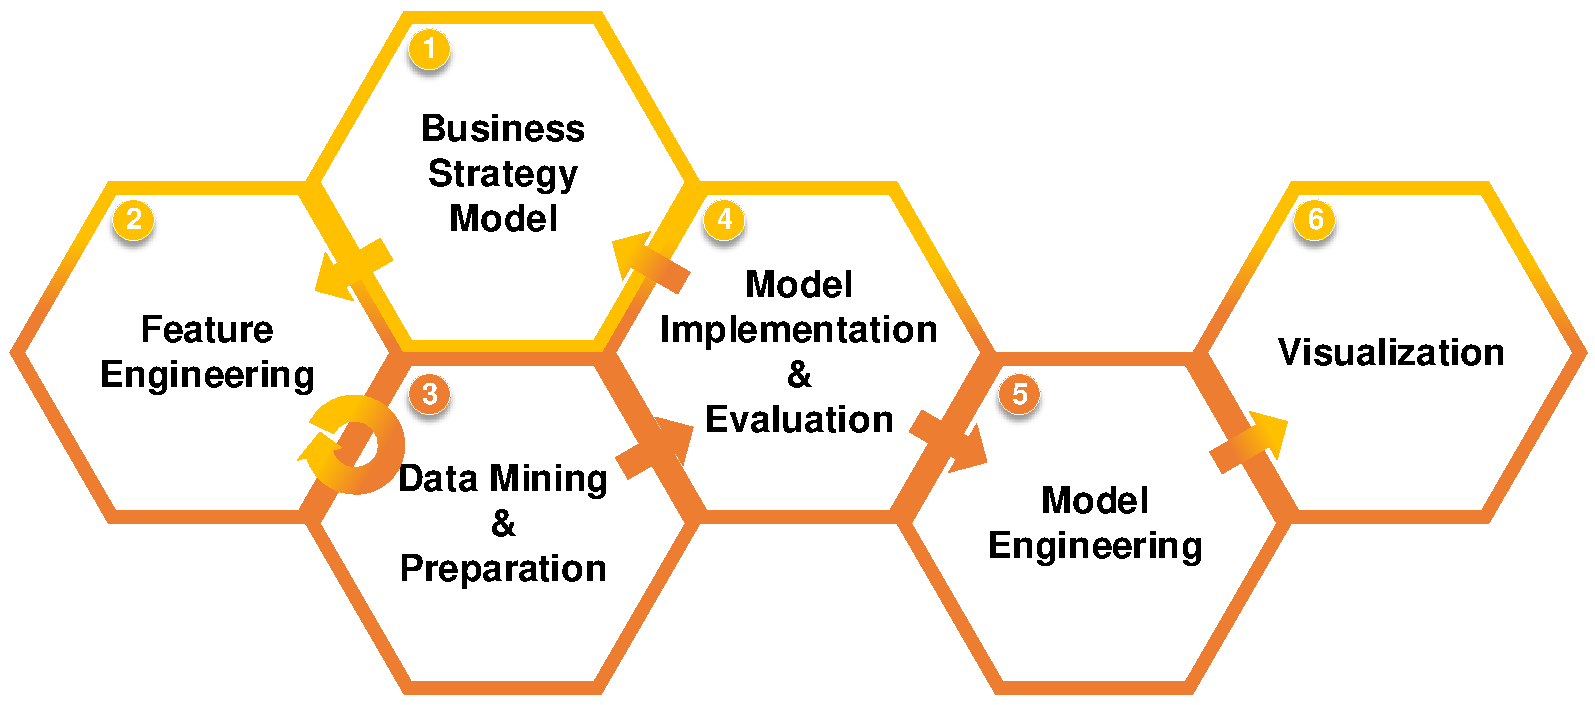
\includegraphics[width=10cm]{contenido/imagenes/DDSD.pdf}
    \caption{Duis tristique velit velit. Curabitur auctor, nibh.}
    \label{fig:figure1}
\end{figure}

%%%                  %%%
% Document structure   %
%%%                  %%%
\section{Estructura del documento}\label{sec:estructura}
Lorem ipsum dolor sit amet \cite{entry2013one}, consectetur adipiscing elit. Phasellus eu risus convallis, cursus ante quis, condimentum nibh. Cras vulputate suscipit tortor eu pulvinar. Aenean aliquet felis lacinia aliquet interdum. In at diam sed lacus porta efficitur. Nunc hendrerit, felis id venenatis fringilla, augue justo egestas ipsum, vel pretium est lorem at arcu. Nullam finibus mauris et maximus viverra. Etiam sagittis ligula vel aliquam vehicula. Aenean consequat condimentum enim, eget posuere lectus dapibus sed. Suspendisse mollis \apa{entry2002two} eu orci eu tempor. Aliquam tempus enim eget egestas congue. Morbi nisi metus, suscipit in scelerisque quis, accumsan sit amet nulla. Sed id imperdiet quam, eget commodo sem. Donec et molestie libero. Donec et quam mi. Vivamus consectetur est turpis, et ultricies leo dictum eu.\par

\begin{itemize}
    \item Lorem ipsum dolor sit amet, consectetur adipiscing elit.
    \item Vestibulum id tortor efficitur odio dictum suscipit ut blandit augue.
    \item Donec consectetur sem ac suscipit bibendum.
    \item Phasellus interdum metus sit amet lorem tempor, vel accumsan mi maximus.
    \item Suspendisse semper massa et porttitor gravida.
    \item Vestibulum vestibulum eros id quam eleifend consequat.
\end{itemize}{}

    
